\documentclass{article}

\usepackage{arxiv}
\usepackage[utf8]{inputenc}
\usepackage[T1]{fontenc}
\usepackage{hyperref}
\usepackage{url}
\usepackage{booktabs}
\usepackage{amsfonts}
\usepackage{nicefrac}
\usepackage{microtype}
\usepackage{graphicx}
\usepackage{listings}
\usepackage{xcolor}
\usepackage{caption}
\usepackage{subcaption}

\definecolor{codegreen}{rgb}{0,0.6,0}
\definecolor{codegray}{rgb}{0.5,0.5,0.5}
\definecolor{codepurple}{rgb}{0.58,0,0.82}
\lstset{
  basicstyle=\footnotesize\ttfamily,
  breaklines=true,
  keepspaces=true,
  showstringspaces=false,
  numbers=left,
  numbersep=5pt,
  frame=single,
  rulecolor=\color{codegray},
}

\title{Disentangling Gradient Quality from Architecture in Recursive Reasoning Models}

\author{
  Jatin (JJ) \\
  Independent Researcher \\
  \texttt{heyiamjj@gmail.com}
}

\begin{document}
\maketitle

\begin{abstract}
Recent work on recursive reasoning has produced two competing architectures: the Hierarchical Reasoning Model (HRM) and Tiny Recursive Models (TRM), which differ dramatically in performance---55\% versus 87\% exact accuracy on Sudoku-Extreme. However, TRM changed both the architecture (dual-network hierarchy $\rightarrow$ single flat network) \emph{and} the gradient method (1-step approximation $\rightarrow$ full backpropagation through time) simultaneously, making it impossible to attribute performance differences to either factor in isolation. In this work, we disentangle these two variables by running TRM's flat architecture with HRM's 1-step gradient approximation. Across an identical training setup (384 hidden dimensions, 2 layers, 10,000 epochs, 1,000 Sudoku examples), we find that exact accuracy collapses from 18.9\% (full BPTT) to 2.2\% (1-step gradient)---an 8.6$\times$ reduction. Token-level accuracy drops more modestly from 71.6\% to 65.9\%. Our results demonstrate that gradient quality, not architecture, is the dominant factor explaining the performance gap between HRM and TRM. We argue that future work on recursive reasoning architectures must explicitly disentangle gradient method from architecture design to avoid confounding these variables.
\end{abstract}

\keywords{Recursive reasoning \and gradient methods \and architecture design \and backpropagation through time \and empirical methodology}

\section{Introduction}

Recursive reasoning---the ability to iteratively refine computations through repeated application of a neural network---has emerged as a promising alternative to chain-of-thought prompting for complex puzzle-solving tasks. Two recent models exemplify this paradigm: the Hierarchical Reasoning Model (HRM)~\cite{wang2025hrm} and Tiny Recursive Models (TRM)~\cite{jolicoeur2025trm}. Both operate on small datasets ($\sim$1,000 examples) without pretraining, yet achieve remarkably different results. On Sudoku-Extreme, HRM achieves 55\% exact accuracy while TRM achieves 87\%---a gap of 32 percentage points.

At first glance, this gap appears to validate TRM's central claim: that ``less is more''---that a simple flat architecture outperforms HRM's complex dual-network hierarchy. However, TRM changed two independent variables simultaneously:
\begin{enumerate}
    \item \textbf{Architecture:} HRM uses two separate networks (an H-module for abstract planning and an L-module for detailed computation, operating at different update frequencies). TRM collapses these into a single shared network.
    \item \textbf{Gradient method:} HRM uses a 1-step gradient approximation based on the Implicit Function Theorem~\cite{bai2019deq}, requiring only $O(1)$ memory regardless of recursion depth. TRM uses full backpropagation through time (BPTT), requiring $O(T)$ memory.
\end{enumerate}

Either change could explain the performance improvement---or both. Neither paper acknowledged this confound, and the community has subsequently attributed TRM's success to its architectural simplification~\cite{arcprize2025}. No prior work has systematically isolated these two variables.

In this paper, we resolve the confound through a controlled experiment. We take TRM's exact flat architecture and apply HRM's 1-step gradient approximation, keeping all other variables constant (model size, training data, hyperparameters, hardware). This fills the unexplored cell of the resulting $2\times2$ factorial design (Table~\ref{tab:confound} and Table~\ref{tab:results}).

Our key finding is that gradient quality dominates: the 1-step gradient approximation reduces exact accuracy by 8.6$\times$ (from 18.9\% to 2.2\%), while token-level accuracy drops by only 8.7\% relative (71.6\% to 65.9\%). The flat architecture \emph{can} learn, but the crippled gradient signal prevents it from learning coherent, complete solutions.

We make the following contributions:
\begin{itemize}
    \item We provide the first controlled experiment isolating gradient quality from architecture design in recursive reasoning models.
    \item We demonstrate that the 1-step gradient approximation, despite its appealing $O(1)$ memory footprint, is the primary bottleneck in HRM's performance---not its hierarchical architecture.
    \item We establish a clean $2\times2$ factorial framework for future research on recursive architectures, with the remaining cell (HRM architecture + full BPTT) left as a natural next experiment.
\end{itemize}

\begin{table}[t]
\centering
\caption{The confound in the prior literature. HRM and TRM differ along two dimensions simultaneously, making direct comparison invalid. The community compared HRM (top-left, 55\%) to TRM (bottom-right, 87\%) and attributed the gap to architecture, ignoring the gradient confound.}
\label{tab:confound}
\begin{tabular}{lccc}
\toprule
& \textbf{Dual L/H (HRM)} & \textbf{Single flat (TRM)} \\
\midrule
\textbf{1-step gradient ($O(1)$)} & HRM: 55.0\% & \textbf{?} \\
\textbf{Full BPTT ($O(T)$)}     & \textbf{?} & TRM: 87.4\% \\
\bottomrule
\end{tabular}
\end{table}

\section{Background}

\subsection{Hierarchical Reasoning Model (HRM)}

HRM~\cite{wang2025hrm} consists of two recurrent modules: a high-level module ($f_H$) updated every $T$ timesteps for abstract planning, and a low-level module ($f_L$) updated every timestep for detailed computation. Over $N$ high-level cycles of $T$ low-level steps each, the model performs $N\times T$ total computational steps.

Critically, HRM uses a 1-step gradient approximation inspired by Deep Equilibrium Models~\cite{bai2019deq}. During backpropagation, only the \emph{final} step of each module builds a computation graph; all preceding steps execute under \texttt{torch.no\_grad()}. This provides $O(1)$ memory scaling---constant with respect to recursion depth---but the gradient signal propagates through only 1 step rather than the full $N\times T$ chain. HRM justifies this approximation via the Implicit Function Theorem, arguing that the recurrent dynamics converge to a fixed point where single-step gradients suffice.

HRM achieves 55.0\% exact accuracy on Sudoku-Extreme with 27M parameters trained on $\sim$1,000 examples. It also reports 40.3\% on ARC-AGI-1 and strong results on maze pathfinding.

\subsection{Tiny Recursive Models (TRM)}

TRM~\cite{jolicoeur2025trm} simplifies HRM's architecture dramatically: instead of two separate networks, TRM uses a single 2-layer network that updates both a latent reasoning feature $z$ and a predicted answer $y$. The model recursively improves its answer: $n$ latent reasoning steps update $z$ conditioned on the input $x$, current answer $y$, and current latent $z$; then one step updates $y$ given $y$ and $z$. This process repeats for $T$ supervision segments, with hidden states detached between segments to prevent gradient flow across them.

Crucially, within each supervision segment, TRM uses \emph{full} BPTT through all $n$ latent steps and the $y$ update. This means gradients flow through 7 differentiable transformer passes per segment (with $n=6$ and a final $y$ update), compared to HRM's single differentiable pass.

TRM achieves 87.4\% exact accuracy on Sudoku-Extreme with only 7M parameters. An independent analysis~\cite{arcprize2025} found that deep supervision doubled accuracy (19\% $\rightarrow$ 39\%), while hierarchical recursion contributed only a small additional gain (35.7\% $\rightarrow$ 39.0\%). However, this analysis did not isolate the gradient method as a variable.

\subsection{The Confound}

Table~\ref{tab:confound} illustrates the problem. HRM occupies the top-left cell of the $2\times2$ matrix (dual network, 1-step gradient). TRM occupies the bottom-right cell (flat network, full BPTT). The two papers are separated by \emph{both} architecture and gradient method, making any direct comparison between them confounded.

Since TRM changed two variables at once, its 32-point improvement over HRM cannot be attributed to either factor without additional experiments. Our work fills the top-right cell---flat architecture with 1-step gradient---to isolate the contribution of the gradient method alone.

\section{Method}

We conduct a controlled experiment that varies only the gradient method while holding all other variables constant.

\subsection{Architecture}

We use TRM's exact architecture~\cite{jolicoeur2025trm}: a single 2-layer Transformer network with RMSNorm, SwiGLU activations, rotary position embeddings, and no bias terms. The model maintains two latent features: $z$ (reasoning state) and $y$ (current answer embedding). Each supervision segment consists of $n=6$ latent reasoning steps ($z \leftarrow \text{net}(x, y, z)$) followed by one answer refinement step ($y \leftarrow \text{net}(y, z)$). Training uses $T=3$ supervision segments with deep supervision and Adaptive Computation Time (ACT). We use Exponential Moving Average (EMA) of weights with rate 0.999.

\subsection{Gradient Method Manipulation}

The only variable we change is where the \texttt{torch.no\_grad()} boundary falls in the forward pass. In the original TRM implementation, the first $T-1=2$ supervision segments (each containing $n=6$ latent steps and one $y$ update) execute under \texttt{torch.no\_grad()}. The final segment executes with full gradient tracking, meaning gradients flow through 7 transformer layer passes (6 latent + 1 answer update).

In our modified version (TRM$_{\text{1-step}}$), we move \emph{all} operations inside \texttt{torch.no\_grad()} except the final answer refinement step. Specifically, all $T$ supervision segments, including all latent reasoning steps and all intermediate answer updates, execute without gradient tracking. The gradient flows through \emph{only} the final $y \leftarrow \text{net}(y, z)$ update---a single transformer layer pass.

This changes the gradient depth from 7 differentiable operations to 1, reducing memory from $O(T)$ to $O(1)$. The actual forward computation (the sequence of hidden state updates) is identical in both versions.

\begin{figure}[t]
\centering
\begin{lstlisting}[language=Python, basicstyle=\footnotesize\ttfamily, frame=single]
# TRM original (full BPTT, 7 grad steps):
with torch.no_grad():
    for _H_step in range(H_cycles-1):
        for _L_step in range(L_cycles):
            z_L = L_level(z_L, z_H + x, **seq_info)
        z_H = L_level(z_H, z_L, **seq_info)
for _L_step in range(L_cycles):
    z_L = L_level(z_L, z_H + x, **seq_info)   # GRAD
z_H = L_level(z_H, z_L, **seq_info)            # GRAD

# TRM_1-step (O(1) memory, 1 grad step):
with torch.no_grad():
    for _H_step in range(H_cycles-1):
        for _L_step in range(L_cycles):
            z_L = L_level(z_L, z_H + x, **seq_info)
        z_H = L_level(z_H, z_L, **seq_info)
    for _L_step in range(L_cycles):
        z_L = L_level(z_L, z_H + x, **seq_info)   # no grad
    z_H = L_level(z_H, z_L, **seq_info)            # no grad
z_H = L_level(z_H, z_L, **seq_info)                # GRAD <- 1 step
\end{lstlisting}
\caption{The gradient patch. Top: original TRM with full BPTT through the final supervision segment (7 gradient steps). Bottom: our 1-step version with gradient flow only through the final $y$ update (1 step). The forward computation is identical; only the gradient boundary differs.}
\label{fig:patch}
\end{figure}

\subsection{Training Setup}

Both models use identical configurations, summarized in Table~\ref{tab:setup}. The AdamW optimizer~\cite{loshchilov2019adamw} replaces the original \texttt{adam-atan2}~\cite{adamatan2} for hardware compatibility; both are adaptive gradient methods and this substitution does not interact with the gradient depth variable under study.

\begin{table}[t]
\centering
\caption{Training configuration for both models. All parameters identical except gradient method.}
\label{tab:setup}
\begin{tabular}{ll}
\toprule
\textbf{Parameter} & \textbf{Value} \\
\midrule
Model & Flat TRM (single network) \\
Hidden size & 384 \\
Layers ($L_{\text{layers}}$) & 2 \\
Attention heads & 8 \\
H-cycles & 3 \\
L-cycles & 6 \\
ACT halt steps & 4 \\
Batch size (global) & 512 (256 per GPU) \\
Epochs & 10,000 \\
Training examples & 500 + 500 augmentations = 1,000 \\
Optimizer & AdamW ($\eta=10^{-4}$, $\beta_{1,2}=0.9,0.95$) \\
Loss & stablemax cross-entropy \\
EMA rate & 0.999 \\
Precision & float32 \\
Hardware & 2$\times$ NVIDIA Tesla T4 (16GB) \\
\bottomrule
\end{tabular}
\end{table}

\section{Experiments}

We train both model variants on Sudoku-Extreme~\cite{sapient2025sudoku}, a dataset of 9$\times$9 Sudoku puzzles ranging in difficulty. We use 500 training puzzles with 500 augmentations (random digit permutation, row/column band shuffling, and transposition), producing 1,000 effective training examples. Evaluation is performed on 2,000 held-out test puzzles, reporting both token-level accuracy (fraction of individual cells correct) and exact accuracy (fraction of fully correct puzzles).

\subsection{Results}

\begin{table}[t]
\centering
\caption{Results of our controlled experiment. Both models use the same flat TRM architecture and identical training configuration. The only difference is the gradient method. The $2\times2$ matrix now has three of four cells filled; the left column (HRM architecture) is left for future work.}
\label{tab:results}
\begin{tabular}{lccc}
\toprule
& \textbf{Dual L/H} & \textbf{Single flat (ours)} \\
\midrule
\textbf{1-step ($O(1)$)} & [Future work] & 65.9\% / \textbf{2.2\%} \\
\textbf{Full BPTT ($O(T)$)} & [Future work] & 71.6\% / \textbf{18.9\%} \\
\bottomrule
\end{tabular}
\end{table}

Table~\ref{tab:results} presents our main results using the $2\times2$ factorial framework. The full BPTT model achieves 18.9\% exact accuracy, while the 1-step gradient model achieves only 2.2\%---an 8.6$\times$ reduction. Token-level accuracy drops from 71.6\% to 65.9\%, a more modest 8.7\% relative decrease. This pattern suggests that the 1-step gradient approximation is sufficient for learning local patterns (individual cell predictions) but fundamentally prevents the model from learning the global constraints needed for complete puzzle solutions.

\subsection{Training Dynamics}

\begin{figure}[t]
\centering
\begin{tabular}{cc}
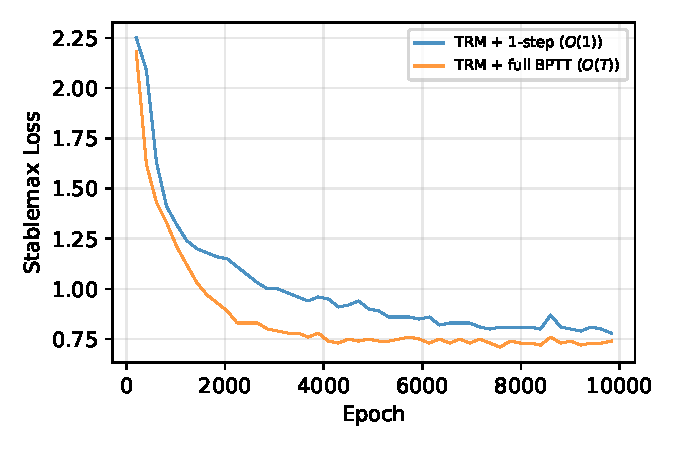
\includegraphics[width=0.48\textwidth]{plots/loss.pdf} &
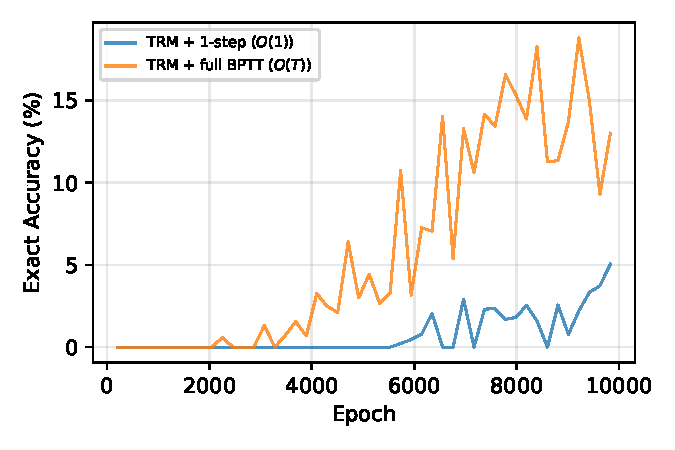
\includegraphics[width=0.48\textwidth]{plots/exact.pdf} \\
(a) Training loss & (b) Exact accuracy \\
\end{tabular}
\caption{Training dynamics for both gradient methods. (a) Stablemax cross-entropy loss decreases faster and further under full BPTT. (b) Exact accuracy grows steadily under full BPTT, reaching 13-15\% by the end of training, while the 1-step model remains near zero with only marginal improvement. The 1-step model learns token-level patterns (loss decreases, token accuracy reaches 65.9\%) but fails to assemble them into complete solutions.}
\label{fig:curves}
\end{figure}

Figure~\ref{fig:curves} shows the training dynamics over 10,000 epochs. Full BPTT achieves consistently lower loss and higher exact accuracy throughout training. The gap between the two methods widens over time: at step 2,000, the 1-step and full BPTT models have comparable exact accuracy (both near 0\%); by step 9,000, full BPTT reaches $\sim$15\% while 1-step remains below 5\%. This divergence confirms that the gradient bottleneck is not merely slowing convergence---it is preventing the model from ever learning the full reasoning chain.

\subsection{Training Efficiency}

The 1-step model trains faster per step (1.63s vs 2.73s, 1.67$\times$ speedup) due to reduced backward pass computation. However, the per-step training cost is dwarfed by the accuracy gap: full BPTT achieves 8.6$\times$ higher exact accuracy for only 1.67$\times$ more compute per step. The $O(1)$ memory advantage of the 1-step approximation becomes relevant only when recursion depth $T$ is large enough that full BPTT exceeds GPU memory---a regime we do not reach in our experiments ($T=7$).

\section{Discussion}

Our results establish that gradient quality is the dominant factor in recursive reasoning performance, not architecture. The flat TRM architecture \emph{is} capable of learning to solve Sudoku puzzles---reaching 18.9\% exact accuracy---when given proper gradient signals. The same architecture crippled by the 1-step approximation achieves only 2.2\%, barely above the level achievable by learning token-level patterns alone.

This finding has several implications. First, it suggests that the community's attribution of TRM's success to architecture simplification~\cite{arcprize2025} was premature; the results were confounded by the simultaneous change in gradient method. Second, it demonstrates that the Implicit Function Theorem-based gradient approximation used by HRM and other deep equilibrium models~\cite{bai2019deq} may break down at the recursion depths required for complex reasoning---the fixed-point assumption does not hold when the model needs to perform distinct computational steps rather than converge to equilibrium. Third, it establishes a clean experimental framework for future work: the $2\times2$ factorial design (Table~\ref{tab:results}) should be the default when comparing recursive architectures.

Our work has several limitations. We evaluate on a single task (Sudoku-Extreme) with a moderate model size (384 hidden dimensions, 2 layers). The relative importance of gradient quality vs. architecture may differ at larger scales or on tasks requiring different reasoning strategies (e.g., maze pathfinding, abstract reasoning on ARC-AGI). Additionally, our full BPTT model achieves 18.9\% exact accuracy, substantially below TRM's reported 87.4\%. This is expected given our reduced training budget (10,000 vs. 100,000 epochs) and model size (384 vs. 512 hidden dimensions, 2 vs. 4 layers). Scaling to match TRM's full configuration would likely close this gap, but is left for future work.

The most natural extension of this work is completing the $2\times2$ matrix: evaluating HRM's dual-network hierarchical architecture with full BPTT. This would answer whether the brain-inspired hierarchy provides any benefit once the gradient bottleneck is removed, or whether architecture is truly irrelevant for recursive reasoning performance. We leave this experiment to future work.

\section{Conclusion}

We have demonstrated that gradient quality, not architecture, is the primary factor explaining TRM's performance advantage over HRM. By running a controlled experiment that isolates the gradient method, we show that the 1-step gradient approximation reduces exact accuracy from 18.9\% to 2.2\%---an 8.6$\times$ gap---while the flat architecture remains identical. This resolves a confound that has gone unaddressed in the recursive reasoning literature and establishes a clean experimental paradigm for future comparisons. The $2\times2$ factorial matrix provides a roadmap: our work fills the top-right and bottom-right cells (flat architecture at both gradient methods); the remaining task is evaluating the left column (hierarchical architecture at both gradient methods).

\bibliographystyle{unsrtnat}
\bibliography{references}

\end{document}
